\chapter{Design}

\section{Framework}
In this section I will outline the design decisions that directly effect only the framework produced.

\subsection{Complex Numbers}
Complex numbers are central to Quantum Computing.
As such, any attempt to simulate the behaviour of a Quantum Circuit must handle complex numbers.

There are really only two ways to handle the existence of complex numbers.
One can represent a complex number explicitly as a pair of floating point numbers, or to encapsulate the representation inside a ``complex number'' data structure.

The framework uses the second of these options and provides the ``Complex'' class.
This was chosen for several reasons.
The primary reason was to reduce the risk of programming errors effecting the simulation.
If complex multiplication, addition and other operations had to be replicated throughout the frameworks codebase, and the codebase of any research work, the likelihood of implementation error is much higher, and the tests required to find the error become more specific.
It is much better software engineering practice to encapsulate the properties, real and imaginary values, and the operations on those properties, arithmetic etc.

A season reason is that after brief research online, there are complex number libraries already available.
This reuse of previously written software can also reduce the likelihood of errors in the code.
This is not necessarily due to the software being written by people that are more intelligent or that are better programmers, or even that the software has been explicitly tested more thoroughly than if I were to write a complex number class.
It is due to the size of the deployment footprint.
The number of times the software has previously been deployed, and therefore the number of times it has been implicitly tested by users.

The third reason is that one of the principles behind producing the framework is the attempt to try standardise the research from different researchers.
Without the provision of this ``Complex'' class one researcher could use Cartesian representation, two floating point values, while a second researcher could use the Polar representation, also two floating point values.
If the documentation of the software produced by the two researchers did not mention the representation used, a third researcher could try combine, or compare, the two pieces of software using the framework.
The third researcher is likely to receive very confusing and highly misleading results.
The provision of a Complex class that is used throughout the framework where complex numbers need to be used will reduce the risk of such an event.

\subsection{Matrices}
As seen in Equation \ref{eq:notexplanded} the application of a quantum gate is simply the application of a unitary operation, represented as a matrix, to a quantum state.
This adds the requirement on the framework to provide a manner in which matrices will be represented.

In a similar way to the complex numbers discussed above, there are two distinct ways the framework could have been designed.
The framework could either use an explicit representation, two-dimensional arrays, or could provide a Matrix data structure.

The framework has been designed to use the data structure encapsulation as the matrix representation.
The justification is identical to that discussed above.
Matrix operations are easy to get wrong in implementation and there are matrix libraries for many languages.
The incomplete documentation argument also holds with matrices.
If the framework were to just simply represent matrices as two dimensional arrays, two researchers could order the dimensions differently leading to similar problems to that of conflicting complex representations for the third researcher.

\subsection{State}
With a representation of matrices defined, the definition of a quantum state naturally followed.
Using the matrix representation, quantum states are defined simply as $2^n\times1$ matrices, vectors.
This representation makes unitary application much simpler as it automatically supported as matrix multiplication.

\subsection{Test Suite Structures}
\label{sec:testsuitestruc}
With most problems there are a series of expected results that are used to measure the suitability of any suggested solution.
The expected results are also usually coupled with the respective inputs.

For Quantum Algorithms the expected results are the state vectors produced by circuits constructed by the algorithm.
As such it was chosen that a test case would be represented as a pair of state vectors, the stating state and the expected state.
The application of a quantum gate is a simple mapping from a starting state to a resulting state.
When a circuit can be defined as a single unitary operation, a custom quantum gate, this representation seems a natural choice.

Each circuit produced by the Quantum Algorithms has $n$ qubits.
This means that it can only be evaluated using test cases for $n$ qubits.
Test cases for any other number of qubits would not produce useful results.
The notion of a test set was introduced to hold all test cases for a specific $n$.
All test cases are held within a test set.

A test suite is used to hold all the test sets produced for the same problem.
There is only one test set for each distinct value of $n$.

The test suite is fully defined in a single XML file.
The XML in Figure \ref{code:paulixtestset} is a sample of such a file.
It is easy to see file structure reflects the internal structure of test suites just described.

\lstset{language = XML}
\begin{figure}
 \begin{lstlisting}
 <testsuite>
    <testset NumQubits="1">
      <testcase><!--0-->
	<starting_state>
	  <matrix_element><!-- 0-->
	    <Real>1.0</Real>
	    <Imag>0.0</Imag>
	  </matrix_element>
	  <matrix_element><!-- 1-->
	    <Real>0.0</Real>
	    <Imag>0.0</Imag>
	  </matrix_element>
	</starting_state>
	<final_state>
	  <matrix_element><!-- 0-->
	    <Real>0.0</Real>
	    <Imag>0.0</Imag>
	  </matrix_element>
	  <matrix_element><!-- 1-->
	    <Real>1.0</Real>
	    <Imag>0.0</Imag>
	  </matrix_element>
	</final_state>
      </testcase>
    </testset>
</testsuite>
 \end{lstlisting}
\label{code:paulixtestset}
\caption{Partial Test Set for Pauli X Gate}
\end{figure}

\subsection{Manager Classes}
As can be seen in the architecture diagram of the framework, Appendix REF???, that there are several classes with names suffixed with ``Manager''.
These classes provide access to the extendible areas of the framework.
There is a Manager class for the Fitness Functions, the Search Engines and the Problems.
Each of these are a specific site of expansion.

Each Manager is configured using an XML file specfying all options for the specific Manager.
The Fitness Function Manager will be configured for all the available Fitness Functions, the Search Engine Manager for all the available Search Engines, and the Problem manager for all the available Problems.

This configuration is performed at runtime rather than at compile time.
it was designed as such so as to provide the ability to add, for example, extra Fitness Functions without altering the code of the framework.
This independence of the framework implementation and the results of research, specific Fitness Funcitons etc, has been identified as one of the key foundations of the framework concept.
The inclusion of this knowledge separation encourages the use of the standardised interfaces specified for each expansion site.

\lstset{language=XML}
\begin{figure}
\begin{lstlisting}
 <FitnessFunc>
	<FitnessFunctionTag>
	  <Name>FITNESS FUNCTION NAME</Name>
	  <Class>IMPLEMENTING FULLY QUALIFIED CLASS NAME</Class>
	  <Desc>FITNESS FUNCTION DESCRIPTION</Desc>
	</FitnessFunctionTag>
</FitnessFunc>
\end{lstlisting}
\caption{XML for Fitness Function Manager Configuration}
\label{code:fitfuntmanconfig}
\end{figure}

The XML outline shown in Figure \ref{code:fitfuntmanconfig} is an outline of the XML file used to specify the available Fitness Functions.
The XML files specifying the available Search Engines and the available Problems can be found in Appendix \ref{sec:semanspecxml} and \ref{sec:probmanspecxml}.

These XML files are used to regiser the available implementations with the respective Managers.
The Manager classes use these registrations to provide the choice of available instantiations of Search Engines, Fitness Functions and Problems.

\subsection{Multiple Search Engines}
The framework is aimed to be used universally by Quantum Algorithm researchers.
The search techniques used by these researchers are also a matter of research effort.
If the tool were to provide a search engine, with no option for change, the use of the tool is likely to be significantly impacted.

Providing a simple interface that allows each researcher to potentially use a different search technique is likely to increase the tools applicability.
The simple interface allows a user to:
\begin{itemize}
 \item retreive the names, used as the search engine identifier, of all registered Search Engines
 \item retreive the instantiation of the specified Search Engine instantiation
 \item retreive the description of the specified Search Engine
\end{itemize}

All registered Search Engines must implement the supplied interface.
The Search Engines are not restricted to evolutionary approaches.
The internal workings of the different search engines are unrestricted.

The alternative approach would have been to implement a series of search engines based on several different techniques and provide researchers this choice.
This was not accepted as it moved the tool away from the framework intended.
The provision of search engines without a simple manner to add additional engines would restrict research and not allow researchers to easily use techniques developed in the research community within the system.

\subsection{Multiple Fitness Functions}
As was noted by Massey\cite{masseythesis}, different Fitness Functions can have a dramatic impact on the success of a Quantum Algorithm search.
The inclusion of a choice of Fitness Functions is to account for this.
As with Search Engines, the choice of Fitness Functions is provided by the Manager class through a simple interface with methods synonomous to those provided for the Search Engine selection.
A Fitness Function interface is provided to ensure that all Fitness Functions are able to be used universally within the tool and are not specific to any particular Search Engine for example.

Similarly to the Search Engine, a series of Fitness Functions could have been implemented and provided without provision for extension.
The justification for the approach taken is the same as listed for the multiple Search Engines.
It was deemed detrimental and in contradiction of the frameworks purpose to limit the Fitness Functions to those provided by the tool.


\subsection{Multiple Problems and Problem Specification}
As has been mentioned on several occasions, one of the foundation principles of the framework is the ability to ``Plug and Play'' the work of other researchers without the proplem of integration.
With Search Engines and Fitness Functions developed to adhere to the respective interfaces, a user should be able to work with the toolkit and treat it as a ``Black Box''.

In Section \ref{sec:testsuitestruc} how test suites and all their contained test cases are specified in XML was described.
The use of XML files does however increase the effort required from the user.
The user needs to specify, each time they use the framework, the location of the XML file containing the correct test suite.
To reduce this effort the problem container is introduced alongside its manager.

The problem manager allows multiple problems to be defined within a single XML file so the user need not provide the test suite XML each time the framework is used.
This single XML file contains the definition of mutiple problems.
An example of these XML files can be seen in Figure \ref{code:probmanconfig}.
A problem has a name, description and file name for the respective test suite XML file.
The name and description are used to provide a human readible explanation of the problem represented by the test suite XML file.
The use of a separate XML file to collate all defined problems makes maintenance much simpler.

Providing a problem manager allows the framework to be used for different problems without having to restart the system and without any external software needing to provide different problems explicitly.

\lstset{language=XML}
\begin{figure}
\begin{lstlisting}
<Problems>
  <prob>
    <Name>Final Pauli X</Name>
    <DefFile>config/finalpaulix.xml</DefFile>
    <Desc>A Pauli X gate on the final Qubit</Desc>
  </prob>
</Problems>
\end{lstlisting}
\caption{XML for Problem Manager Configuration}
\label{code:probmanconfig}
\end{figure}

\subsection{Quantum Algorithms}
The result of the search engines are quantum algorithms.
To maintain the ``Plug and Play'' nature of the framework, the representation of these algorithms needed to be specifed and standardised.
However, the representation also had to ensure that it was not limiting the search engines.

To provide a standardised and non-limiting represenation the framework provides an internal quantum algorithm structure that can be simply built by any search engine.
This allows the search engines to have a different internal representation that is then used to build the standardised algorithm.
Using this there are no limitations on the structures used internal to the search engines.

The use of the standardised quantum algorithm also ensures that the reporting of an algorithm to the user is consistent.

\subsection{Qubit Numbering}
One of the major decisions made relating to the way in which the produced quantum algorithms are produced was that of which way the qubits should be numbered.
The two options were obviously in accending or decending order.

The chosen approach was the decending order.
This meant that for state $\ket{ab{\dots}st}$ the qubit represented by $a$ would always be given the identifier equal to the number of qubits in the system.
For example, if there were three qubits in the system the identifier of the qubit represented by $a$ would be $3$.
This was chosen to ensure that an identifier always represented the same qubit, irrespective of the number of qubits in the system.

The justification for this is to make the algorithm much more understandable.
If the identifers were dependant on the number of qubits it would make the results of the system much less comprehensible.

The use of this numbering is also much more natural as the identifer, $x$, of a qubit, $a$, is related to the value of the qubit when read in binary.
The value of the qubit $a$ is $2^{x-1}$.
This makes the optimisation of gate application, see Section \ref{sec:quantumgates}, much simpler.

\subsection{Quantum Circuits}
To perform the evaluation of an algorithm the circuits for the test sets need to be produced.
Both the representation of the circuit and the mechanism to construct the circuit from the algorithm needed to be standardised to ensure the ``Plug and Play'' nature of the framework.

The framework provides a default circuit builder.
The framework does allow a separate circuit builder to be provided as long as it conforms to the interface and the circuits it produces also adheres to the respective interface.
There is no manager class provided for circuit builders.
This was due to an assessment of the intended uses of the framework.
It is intended that the framework would be used primarily to perform the following:
\begin{itemize}
  \item Perform research into the effect of different fitness functions on the search for quantum algorithms
  \item Perform research into different search techniques that could be used to produce quantum algorithms
  \item Perform research to produce new quantum algorithms for a specific problem
\end{itemize}

It is not seen as a priority of the system to provide the same level of flexibility to the circuit building as the search engines and fitness functions.

The circuits that are produced by a circuit builder are hidden behind an interface.
This is to allow third party circuit builders to use their own internal representation and also to allow any future optimisations made in future work on this framework to be made without impacting the work of researchers.

The circuits produced provide the represented quantum circuit as an ordered iterator of quantum gates.
The use of an ordered iterator rather than a specific data structure is to ensure that any future optimisation or third party circuit representation is not limited.
It also reduced the potential errors involving the interpretation of a more complex data structure.

The circuits also provide a Latex representation to allow the circuit to be visualised.
The Latex representation uses the QCircuit package that can be freely obtained at \cite{QCsite}.

\subsection{Quantum Gates}
\label{sec:quantumgates}
Any quantum circuit will be a series of quantum gates on specified qubits.
The quantum gates provided by the system are hidden behind an interface.
This is to ensure that any future optimisation of any gate's implementation cannot interfere with the implementation of any other component of the system.

Each quantum gate is required to provide a unitary matrix but it is not required that the matrix must be used in the application of the gate.
For quantum circuits with a high number of qubits, the cost of simulation increases rapidly.
This is mainly due to the increase in state vector and unitary matrix sizes.
Matrix multiplication is used to apply a unitary operation to a state vector, yet it is a very expensive operation.

To improve the performance optimisations can be applied for several gate types.
This is most obvious when analysing the operation of the Pauli X gate.
Figure \ref{eq:paulixcheaptrickvisual} shows, with the help of colour, that the application of a Pauli X gate on Qubit 1 is essentially a flip of neighbouring values.
This is also true for a Pauli X gate on any other qubit, just the definition of a state's ``neighbour'' is modifed with respect to the identifier of the qubit on which the gate is applied.

\begin{figure}
\[
\begin{tabular}{ r c l }
  \(\begin {pmatrix}
    \textcolor{blue}{a}\\
    \textcolor{red}{b}
  \end{pmatrix}\) 
& 
  \(\rightarrow\) 
& 
  \(\begin {pmatrix}
    \textcolor{red}{b}\\
    \textcolor{blue}{a}
  \end{pmatrix}\) \\

\\

  \(\begin {pmatrix}
    \textcolor{blue}{a}\\
    \textcolor{red}{b}\\
    \textcolor{green}{c}\\
    \textcolor{cyan}{d}
  \end{pmatrix}\)
  & \(\rightarrow\)
  & \(\begin {pmatrix}
    \textcolor{red}{b}\\
    \textcolor{blue}{a}\\
    \textcolor{cyan}{d}\\
    \textcolor{green}{c}
  \end{pmatrix}\) \\
\end{tabular}
\]
\label{eq:paulixcheaptrickvisual}
\caption{Visual Representation of Bit Manipulation Equivelent of Pauli X Operation on Qubit 1}
\end{figure}

The use of these tricks is not specified but the interface has been designed to ensure that the gate implementations can use such tricks or matrix multiplication interchangeably.

Each gate must also provide a QCircuit represenation for use by the circuit to produce the QCircuit representation of the complete circuit.

The implementation of gates effecting two qubits are hidden by an extended interface to provide access to the identifier of the second qubit but ensures that all standard gate operations are also available.

% \subsection{Custom Gates}
% 
% 
% To allow users to introduce their own gates a limited number of custom gates can be included.
% Is limited due to the use of enumeration types in the specification of algorithms.
% Custom gates are like any other gate, a class implementing the correct interface, are specifed through xml specification.

\subsection{Search Engine Parameters}
With many search techniques there are a number of parameters that can be configured and altered, sometimes having dramatic effects on the search results.
To enable the configuration of these parameters through the framework a suitable, and flexible method had to be introduced into the design.
Not all search techniques have the same number of parameters to configure and due to search engines being developed potentially by different researchers, even if the parameters are the same, their internal representation may be different.
To ensure that all parameters that any particular search engine requires can be configured, the user interface for the configuration is provided by the search engine.
The user interface is set to be an onscreen dialog box to ensure that the configuration is controlled by the search engine rather than any third party software or the framework.

This option was chosen as it is fair to assume that the person with best understanding of the parameters provided by a search engine is the same person who implemented the search engine using the parameters.
It therefore follows that to reduce the risk of misunderstanding between GUI developers and search engine developers, who could be spacially and temporally separated, the search engine configuration should be tightly maintained within the search engine implementation.

A second justification for this based on the ``Plug and Play'' nature that is a foundataion of the framework.
If the configuration were provided by third party software providing a GUI for the framework, or embedding it in a larger software suite, the third party software would have to be adapted for each search engine implementation.
This would not be acceptable and is totally against the motivation behind the framework.
With such a design it is likely that the research community would see no advantage to using the framwork than working as they are now, in complete isolation.


\subsection{Design as a Black Box}
The framework is design to be used as a black box.
All external code is only allowed access through the use of interfaces and final or abstract class types.
The implementation of the internal framework functionality is hidden and not required by third party software.
This desgin ensures that third party software shall be loosely coupled with the framework.
\subsection{Interactive Circuit Evaluator}

\section{Provided GUI}

\subsection{GUI Design}
To design the GUI I used the following principles:
\begin{itemize}
 \item \textbf{The structure principle:} Design should organize the user interface purposefully, in meaningful and useful ways based on clear, consistent models that are apparent and recognizable to users, putting related things together and separating unrelated things, differentiating dissimilar things and making similar things resemble one another. 
The structure principle is concerned with overall user interface architecture.
\item \textbf{The simplicity principle:} The design should make simple, common tasks easy, communicating clearly and simply in the user's own language, and providing good shortcuts that are meaningfully related to longer procedures.
\item \textbf{The visibility principle:} The design should make all needed options and materials for a given task visible without distracting the user with extraneous or redundant information. 
Good designs don't overwhelm users with alternatives or confuse with unneeded information.
\item \textbf{The feedback principle:} The design should keep users informed of actions or interpretations, changes of state or condition, and errors or exceptions that are relevant and of interest to the user through clear, concise, and unambiguous language familiar to users.
\item \textbf{The tolerance principle:} The design should be flexible and tolerant, reducing the cost of mistakes and misuse by allowing undoing and redoing, while also preventing errors wherever possible by tolerating varied inputs and sequences and by interpreting all reasonable actions.
\item \textbf{The reuse principle:} The design should reuse internal and external components and behaviors, maintaining consistency with purpose rather than merely arbitrary consistency, thus reducing the need for users to rethink and remember.
\end{itemize}
Taken directly from REFERENCE.

The design of the main sceen of the GUI can be seen in Figure \ref{fig:MainGUIDesign}.
The figure shows the main screen after a a search has been completed.

\begin{figure}
 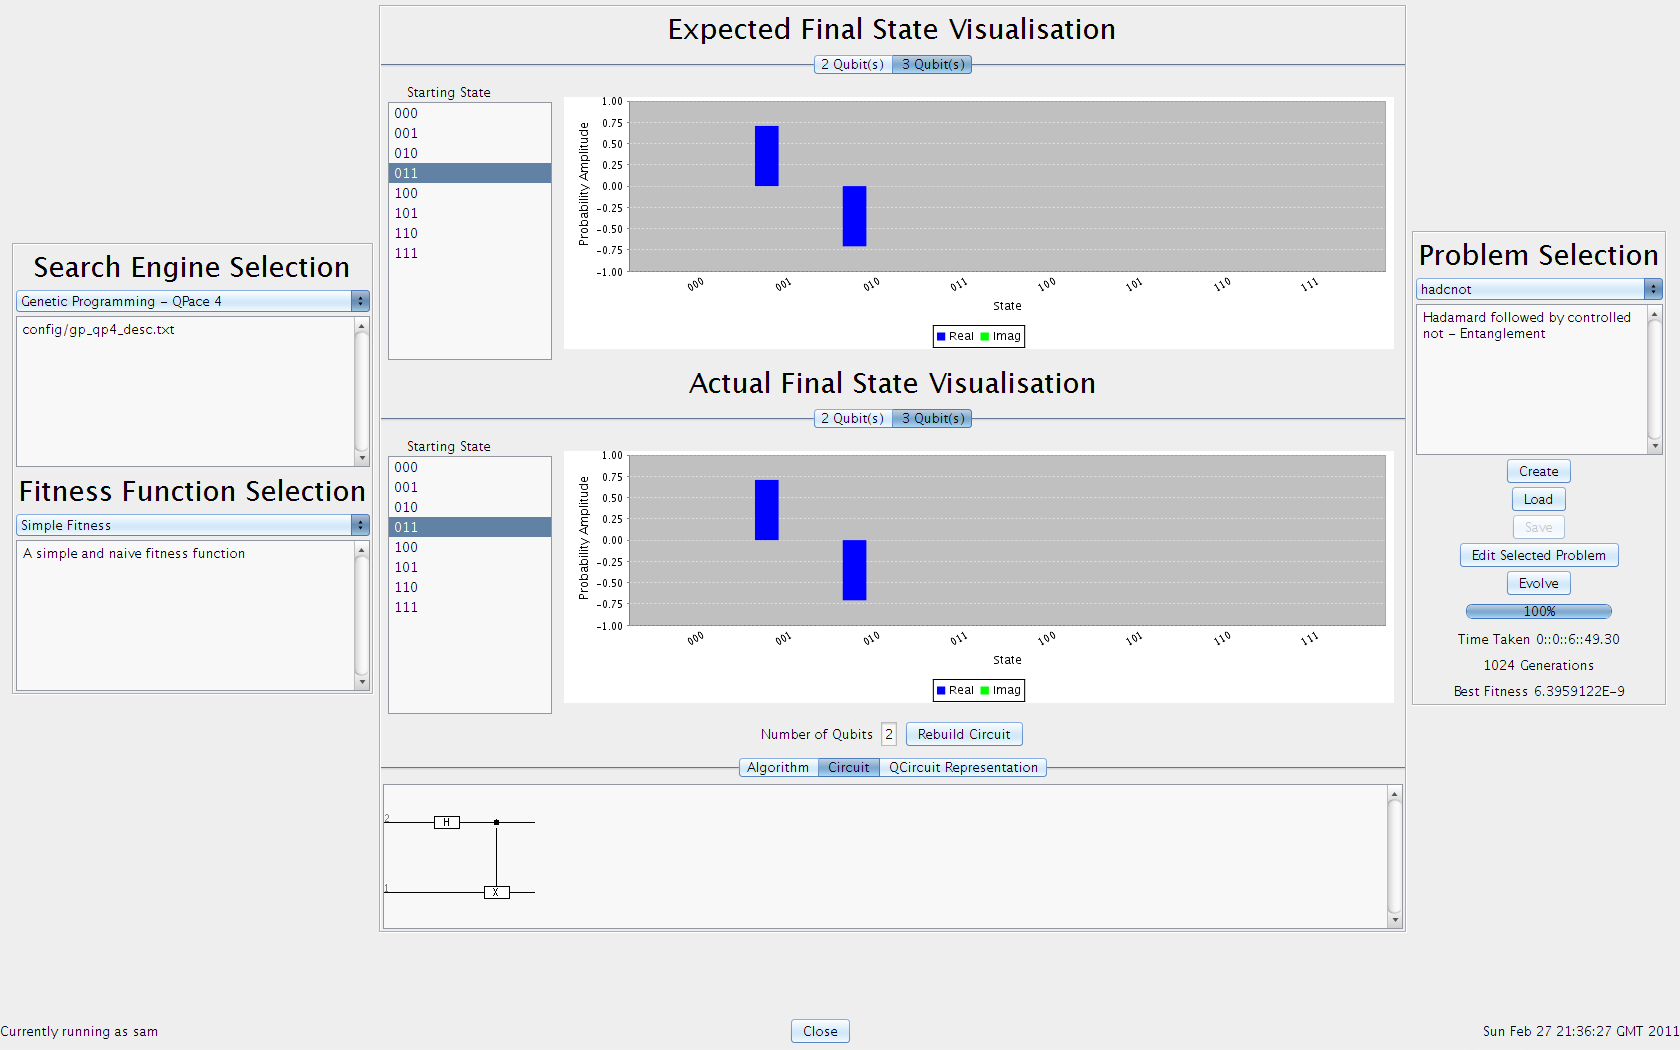
\includegraphics[width=\textwidth]{GUIDesign.png}
\caption{Main User Interface}
\label{fig:MainGUIDesign}
\end{figure}

The justification of the GUI design is broken down with respect to the priciples previously mentioned.

\subsubsection{The Structure Principle}
As can be seen in Figure\ref{fig:MainGUIDesign} the layout separates the ``dissimilar things'' with the use of headings and borders.
The interface can be viewed as structued so that the centre of the display contains the information of the highest importance, straffed by two control menus.
This central panel collates all of the information regarding the result of the latest search.
Visualisation of similar information is shown using the same techniques.
The use of tabs is two-fold.
In the column chart panels it is used to select the data to show using the chart.
In the lowest panel it is used to switch between the different representations of the solution that the system provides.

\subsubsection{The Simplicity Principle}
The way in which the framework has been designed aids in making the user interface simple.
The framework requires very little configuration.
The only real configuration that is required is the selection of which search engine and suitability measure to use and what problem you want to try solve.
These selections are provided in very simple drop down lists for the users seletion.

The only other two aspects of the configuration are the problem editor and the configuration of the search parameters.
These are justified separately.

\subsubsection{The Visibility Principle}
I think it is quite clear to see that the number of ``options'' visible to the user at any one time is minimised.
The use of drop down boxes for selection naturally hides unwanted options until required.

In the central area the available selections are visible but are also much more likely to be ``browsed'' by the user.
The decision not to use drop down boxes for the initial state selection is due to the expected ``browsing'' of this data.
I expect that the user is likely to flick through the various options available which is much easier when the options are always visible.
The use of a drop down box would also have required two mouse clicks per selection, one to open the list and one to make the selection.
With the options visible this is reduced to a single click.

\subsubsection{The Feedback Principle}
Once a selection is made for any of the selections available to the user the information on the display is updated accordingly.
For example, the selection of a different search engine will update the contents of the search engine description area, selecting a different ``input state'' in the graph panels automatically updates the graph and the selection is highlighted.

\begin{figure}
 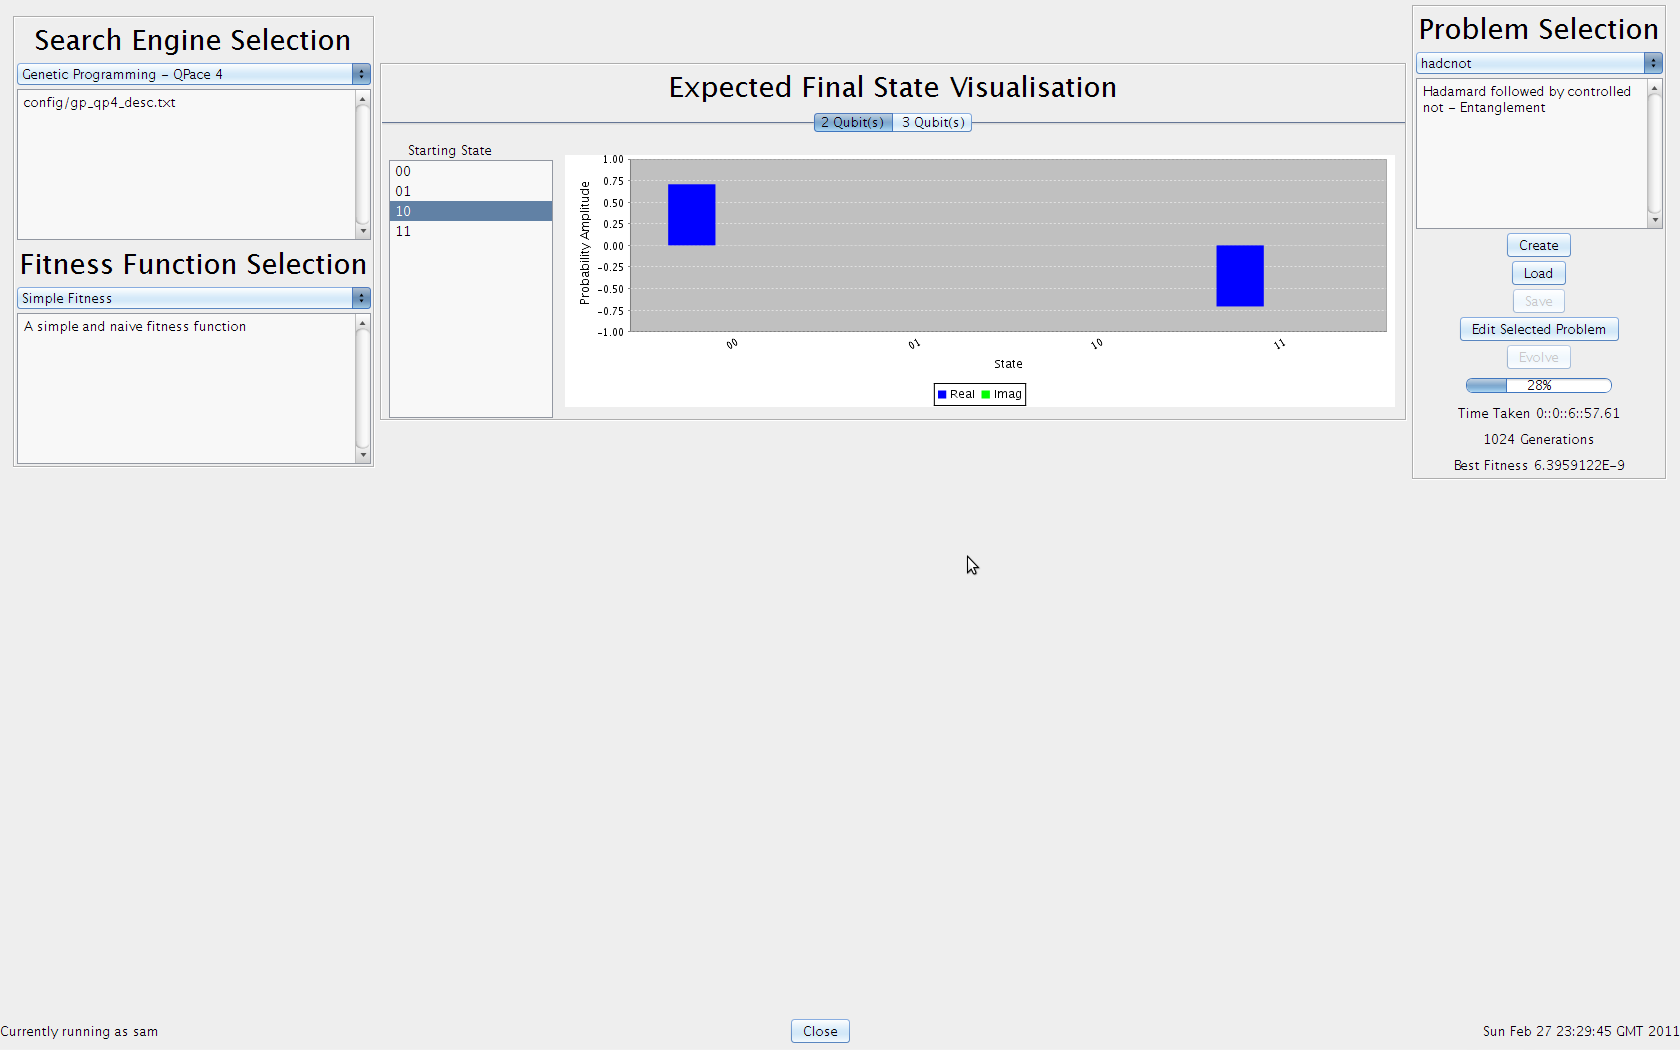
\includegraphics[width=\textwidth]{GUIDesignProgress.png}
\caption{Main User Interface}
\label{fig:MainGUIDesignProg}
\end{figure}

The user interface has been designed so that one user could leave it, a second user come to use it and understand very quickly the decisions that had already been made.
It is not just the selection choices that are provided to the user as feedback.
As can be seen in Figure \ref{fig:MainGUIDesignProg}, a progress bar is provided to indicate to the user how far through the current search the system is.

\subsubsection{The Tolerance Principle}
\subsubsection{The Reuse Principle}

\subsection{Search and Problem Selection}



\subsection{Test Suite Editor}



\begin{itemize}
 \item Extendible Library
\end{itemize}